\subsection{Synthetic validation}
On controlled data with a known dipole and injected non-dipolar content of energy
$\delta$, all three claims hold exactly (Fig.~\ref{fig:synth}). Tier~I error grows
linearly with noise at slope $\|\bm M_s\bm M_{s,S}^{+}\|_F$, and a collinear triplet
($\kappa{=}204$) is far worse than a spread one ($\kappa{=}15$). On Tier~III the
Bayes-optimal estimator's error equals the $\mathrm{Var}(\bm u)$ lower bound at every
$\delta$, while a hallucinator that injects realistic content doubles the error. The
flag's false-flag rate is $0.099{\le}\alpha{=}0.1$ with power reaching $1.0$ for any
non-trivial $\delta$, and Mondrian-CQR attains $0.90$ coverage.

\begin{figure}[t]
  \centering
  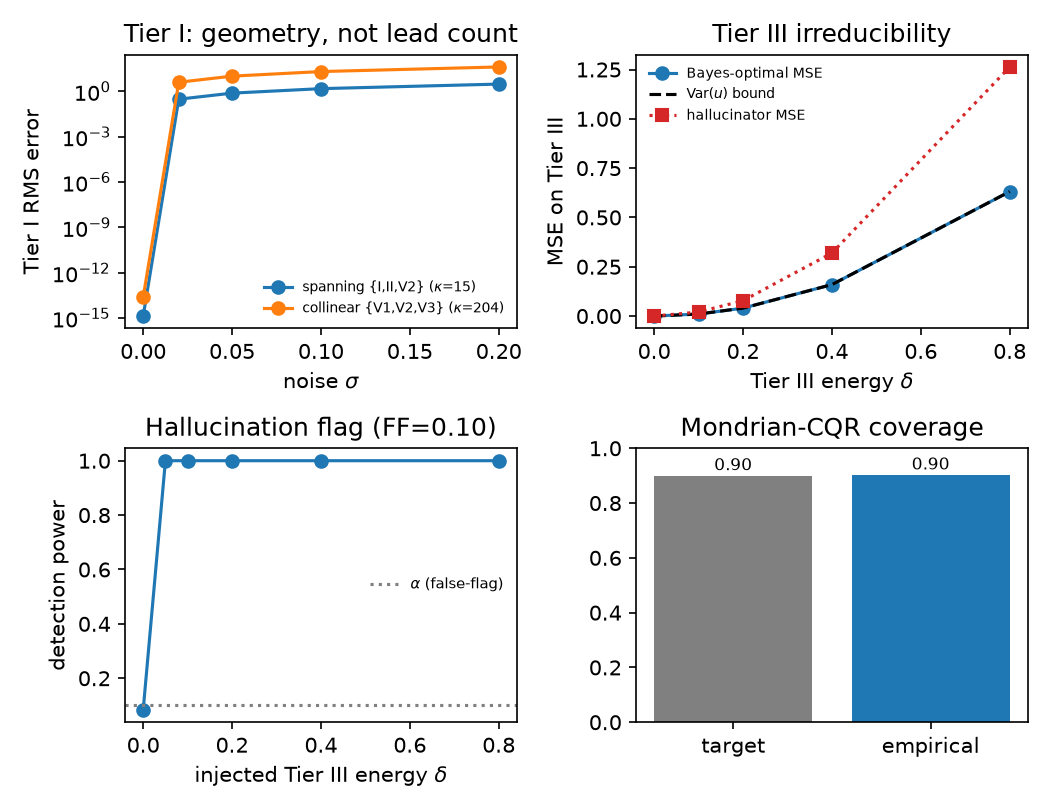
\includegraphics[width=\linewidth]{../results/synthetic_validation.png}
  \caption{Synthetic validation. Tier~I noise gain ($\kappa$); Tier~III
  irreducibility (Bayes $=\mathrm{Var}(\bm u)$; hallucinator $2\times$); flag power
  vs.\ false-flag rate; group-conditional coverage.}
  \label{fig:synth}
\end{figure}
